% !TEX root = template.tex

\section{Processing Pipeline}
\label{sec:processing_architecture}

\begin{figure*}[h]
	\centering
	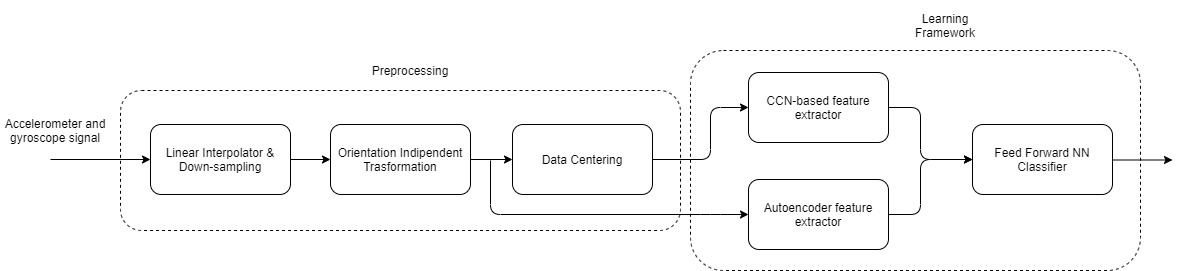
\includegraphics[width=1\textwidth]{images/processing_pipeline.jpg}
	\caption{Processing pipeline}
\end{figure*}

The task of HAR in real use case scenarios is a difficult task, and many aspects need to be considered when these applications are brought in a mobile environment. As reported in \cite{blunck2013heterogeneity} the three major types of heterogeneties which yield impairments in HAR are:
\begin{itemize}
	\item \textbf{Sensor Biases}: To keep the overall cost of a smartphone low, low costs accelerometer and gyroscope sensor are used, yielding a poor-calibrated, inaccurate an of limited granularity and range acquired signals. So, among this type of sensors we could observe differences in precision, resolution, range and also biases. Usually an initial sensors calibration are made by smartphones manufactures, but due to rotation or misalignment of the sensor to the circuit board of the final product, this could introduce errors. Furthermore, if a device experience shock, e.g falling on the ground, the sensor can be misaligned causing unwanted biases.
	\item \textbf{Sampling Rate Heterogeneity}: Often popular smartphones vary in terms of the default and supported sampling frequencies for accelerometer and gyroscope sensor. In the dataset TODO riportare link used for this experiment for example we are dealing with smartphone where the sampling frequency varies from 50Hz to 200Hz. See Fig. TODO so the actual number of devices used in this dataset, with their corresponding sampling frequencies.
	\item \textbf{Sampling Rate Instability}: This phenomenon is specific to a single device and regards the regularity of time span between successive measurements. Different factors could accentuate this problem, including heavy multitasking or high I/O load in the mobile device. Multitasking effect in particular is a major problem: smartphone usually prioritizes among various running tasks and doing so could extremely affects the sensor sampling of a HAR application running on the device. In our collected dataset with a 100 Hz sampling rate,for example we observe a time span between consecutive measurement of TODO, even if the smartphone was hold in \textit{airplane mode} to reduce at the minimum this effect. The Fig. TODO shows the amount of different time-span present in our dataset.
\end{itemize}

Furthermore, if we considered a real use case scenarios of a HAR mobile application we must also consider that smartphones can be positioned and oriented in different ways in human body. For example a smartphone could lay in trouser pockets (back and front) or maybe inside accessories like in a pouch or in a bag with different orientations. These different initial model settings have huge effects in prediction accuracy of an HAR predictor, especially if the model has been trained on a dataset that consist of activity measurement coming from only one fixed position and orientation of the smartphone, as is usually the case dealing with dataset collected in a controlled environment that could be found on Internet. 

To tackle all these problems we decided to adopt in our pre-processing pipeline as show in Fig. TODO, 3 main blocks.

The first block called Linear Interpolator is in charge of mitigate the problems regarding the Sampling Rate Heterogeneity and Sampling Rate Instabilities as discussed previously. It main purpose is to down-sample the input data to a fixed sampling rate, in our case 50 samples/second. 

The second block called Orientation Independent Transformation is used to represent data coming from different orientation of the smartphone in a rotation independent space. In this way all the signals are projected in a new space whose orientation is independent of that of the smartphone and aligned with gravity and the direction of motion. In this way an user can place his smartphone in whatever position he or she wants, mitigating the problem of different position and rotations of smartphone, as we will see in the Experiment section TODO reference.

Our last block consists of a data centering operation, applied for centering signals among y-axis that are presented only for the Covolutional Layer and not for the Autoencoder block. The reason of this choice would be clear in the section TODO. As reported in \cite{ignatov2018real}, time series centering standardize the input data, making the task for the CNN easier. Data normalization instead must be avoided because does not help in this situation since it significantly distorts time series shape, removing magnitude information which is critical for activities differentiation.

After the preprocessing pipeline we adopt a novel Learning framework. It is composed of CNN augmented with features coming from an autoencoder. As discussed in \cite{ignatov2018real} CNNs learns filters that are applied to small sub-regions of the data, and therefore they are able to capture local data pattern and their variations. Additionally, due to a small number of connections and high parallelism the amount of computations and running time of CNNs is significantly lower compared to other deep learning algorithm. This yield these model perfect for real-time HAR apps, where these models could also run in a restrict environment as one like smartphones where computation resources are limited. The only drawback of CCNs is that they fall behind in capturing global properties of the signal, and as proposed in \cite{ignatov2018real} they resolve this problem by augmenting CNNs with some basic statistical features that comprise this aspects of the data. But as opposed to what done in this latter work, where they used manual extracted features, we decided to opt for a autoencoder features extractors which can provide more robust feature. For this reason we train an auto-encoder separately on the training data and then use the encoder part to augment the CNN features used for the last classification Feed Forward Neural Network. 

\section{Signals and Features}
\label{sec:model}

Parlare del nostro dataset usato Heterogenity, cioe come sono strutturati i nostri dati partenza. 



\subsection{Dataset \& Meausurement Setup}
\label{subsec:dataset-measurement-setup}
Parlare di come abbiamo splittato il dataset, quindi escludendo gli utenti a e b per fare in modo di testare le performance cambiando compltamente utente.

Introduzione e spiegazione del dataset eterogeneo, preso da: riportare link. e riportare come abbiamo tirato fuori le time window con overlapping window!

Accenare dell'acquisizione di un nostro dataset alla stessa maniera, a 100 HZ in varie posizioni per testare poi anche tutto il dataset!

\subsection{Signal preprocessing}

In questo caso si va nel dettaglio (con formule e forse se neccessario anche grafici) della parte di preprocessing (parte trattegiata nel mio schema come preprocessing):

\newcommand*{\x}{\boldsymbol{x}}
\newcommand*{\y}{\boldsymbol{y}}
\newcommand*{\z}{\boldsymbol{z}}
\newcommand*{\xm}{\bar{\x}}

As described in Sec. \ref{subsec:dataset-measurement-setup}, our
dataset is composed by signals collected with different sampling rates
from many mobile phones and they are usually out of sync due to the
sampling rate instability. For this reason we apply to all signals a
simple preprocessing pipeline composed by two steps: linear
interpolation and downsampling. With linear interpolation we project
signals with different sampling frequencies, i.e 50, 100, 200 Hz, to a
200 Hz signal. Linear/nearest interpolation are usually preferred
w.r.t. cubic spline or smooth cubic spline as investigated in
\cite{stisen2015smart}, because they usually mitigate the introduction
of noise or artifacts. In linear interpolation the value at time $t$
is the piecewise-linear interpolation, i.e. the linear interpolation
between the input samples adjacent to $t$ in the sequence of input
sample timestamps. Let $(x_0, y_0)$ and $(x_1, y_1)$ be two known
points, the linear interpolant is the straight line between this
points. For a value $x$ in the interval $(x_0, x_1)$ the value $y$
along the straight line is given from the equation of slopes
\begin{equation}
  \label{eq:linear-interpolation}
  \frac{y - y_0}{x - x_0} = \frac{y_1 - y_0}{x_1 - x_0}.
\end{equation}
It's straightforward now to see that if we need to apply linear
interpolation to a dataset of points we can calcultate the $x$-s given
by sampling fraquency we want to obtain and then apply the formula
above. 

At this point we are ready to downsample. Downsampling allows to
standardize data at fixed sampling frequency in order to extract then
time windows and feature vectors for learning models and, above all,
it reduces noise and artifacts introduced by upsampling. Downsampling
simply disregards points by resampling the signal at a lower frequency
(50 Hz in our case). \footnote{FIXME: Please note that the downsample
  frequency should be a sub-multiple of linear interpolation frequency
  otherwise we could}

OIT BRYAN

The last signal processing we perform on the input signal is data
centering. As proved in \cite{ignatov2018real} this could slightly
improve performance within a CNN based learning model because
centering the time series make the task easier for the CNN. We can
define a function $c$ to center a vector
\begin{equation}
  \label{eq:centering-func}
  c(\x) = \x - \xm.
\end{equation}
Centering is applied for each time-window only on accelerometer data, thus
\begin{equation}
  \label{eq:centering-accelerometer-data}
  \boldsymbol{a}_{d}^{c} = c(\boldsymbol{a}_{d})
\end{equation}
where $d = \{ \x, \y, \z \}$. Please note that we simply apply
centering and not normalization which is common in CNN applications
normalization removes relevant information like magnitude which is
critical for activities differentiation.

\subsection{Feature vector}
\begin{itemize}
	\item window strategy
	\item basic feature extraction
	\item autoencoder feature extraction
\end{itemize}

\section{Learning Framework}
\label{sec:learning_framework}

\begin{figure*}[h]
	\centering
	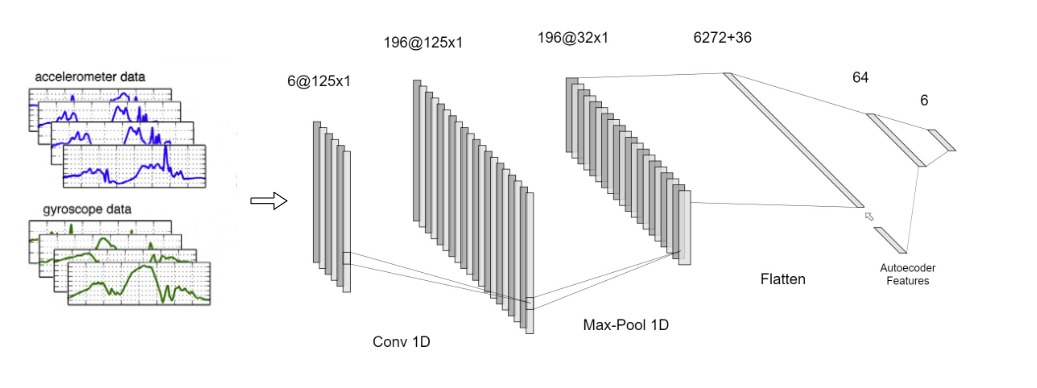
\includegraphics[width=1\textwidth]{images/full_architecture.jpg}
	\caption{Learning Framework}
\end{figure*}

Desctivere qui invece la parte tratteggiata come learning framework

Descivere prima l'autoencoder, come è stato costruito e come viene allenato. TODO luca

Passare alla decrizione della mia archittetura, come sono stai selezionati gli iper-parametri, ecc ecc.

